% Goal: Draft the manuscript for a conceptual framework paper on how the current framework for ecosystem services doesn't capture the dynamics of urban ecosystem services and thus misses how to properly manage them
% Andie Creel / Started November 2026
%
% Goal journal is PNAS. Secondary goal would be something in the Nature family of journals. Another option is Ambio. 

\documentclass[12pt]{article}

% Language setting
\usepackage[english]{babel}

% Set page size and margins
\usepackage[letterpaper,top=2cm,bottom=2cm,left=3cm,right=3cm,marginparwidth=1.75cm]{geometry}

% Useful packages
\usepackage{amsmath}
\usepackage{amssymb}
\usepackage{graphicx}
\usepackage[table]{xcolor} % \rowcolors for shaded table rows (load before tikz)
\usepackage{tikz}
\usetikzlibrary{arrows.meta, decorations.pathreplacing, positioning, fit, backgrounds}
\usepackage{array}
\usepackage{booktabs}
\usepackage{caption}
\usepackage{ragged2e} % for \justifying in table notes
\usepackage{todonotes} % for making comments
\usepackage{natbib}
\usepackage{xurl} % lets long URLs in the bibliography break across lines
\usepackage[colorlinks=true, allcolors=blue]{hyperref}

% Usage: \rev{Author}{comment text}
\newcommand{\rev}[2]{\todo[inline, size=\small, color=yellow!40]{\textbf{#1:} #2}}


\title{A Conceptual Framework of Valuing Urban Ecosystem Services for Decision-Making}
\author{authors}
\date{\today}

\begin{document}
\maketitle

\begin{abstract}
\footnotesize
Existing frameworks describe how urban nature produces value and acknowledge that society responds, but they do not specify who decides, what they are managing for, or what information about benefits they would need to choose a different management plan. Those three missing components -- who decides, what they manage for, and what information they need -- determine whether a city ends up with more natural assets or fewer. This paper proposes a conceptual framework that explicitly incorporates these elements with the goal of setting up a research agenda that will lead to more data-driven decision-making that improves welfare outcomes through well-informed management of urban natural assets.
\end{abstract}



% ------------------------------------------------------------------------------
% Introduction and Motivation of the Paper 
\section{Why Study Ecosystem Services in Urbanizing Places}\label{sec:intro}
% ------------------------------------------------------------------------------
Why is it important to focus on urban/urbanizing areas, and why is it particularly relevant now?
\begin{itemize}
  \item Sheer number of people in urban areas and the rapid pace of urbanization
  \item Climate change has unique dynamics in cities 
  \item Value of ecosystem services \textit{to people} is uniquely important in cities because essentially all of the land and water is managed by people. 
  \begin{itemize}
    \item Decision-makers in cities -- whether its city government, urban planner, business owner, or home owner -- have limited capacity and financial resources to manage ecosystem services in conjunction with all other management responsibilities
    \item Decision makers fundamentally affect the provision and quality of ecosystem services in a unique way in urban environments because the whole urban environment is managed by people, and their decisions directly shape the availability and condition of these services.
    \item Management decisions affect \textit{how} people interact with ecosystem services and \textit{who} benefits from them 
    \item There are many decision-makers in a city, not one. Each considers a single (or subset) of the potential benefits natural assets provide (e.g., a storefront sees revenue, an insurer sees claims, a city sees its budget), and the one who benefits may not control the asset
    \item \textbf{Andie: this sets up our contribution in the CF section. The framework is organized around the decision, not the ecosystem: who can change the stock of natural assets, what they are managing for, and what measured benefit would change their choice.}
  \end{itemize}

% ------------------------------------------------------------------------------
% Introduction and Motivation of the Paper 
\section{What is Unique about Ecosystem Services in Urban/Urbanizing Areas}\label{sec:background}
% ------------------------------------------------------------------------------


  \textbf{Andie: Originally we wanted below to sit under this second section, but it seems like maybe the Section \ref{sec:intro} could be combined with Section \ref{sec:background}}

  \item Urban areas are rapidly growing and an constant flux of development and demographic change, which creates dynamic challenges and opportunities 
  \begin{itemize}
    \item Rapid urban growth leads to greater pressure to develop existing natural resources
    \item Demographic changes, such as population density and diversity, influence the types of ecosystem services needed and valued by urban residents
    \item Cities that have are already built-up face challenges in maintaining and enhancing ecosystem services amidst already limited available space 
    \item Cities that are still expanding should have a forward looking planning approach to preserve/conserve urban natural assets in present day while facing tremendous development pressures. To do so, decision makers will need to understand the value of conserving/preserving natural assets in comparison to those development alternatives.
  \end{itemize}
  \item Some simple table emphasizing the differences between urban and non-urban ecosystem services contexts (Table~\ref{tab:urban_vs_nonurban}) 
  
  \begin{table}[h!]
    \centering
    \caption{[DRAFT] Comparison of Urban and Non-Urban Ecosystem Service Contexts}
    \rowcolors{2}{white}{gray!12} % alternate grey rows in the body (header is row 1)
    \begin{tabular}{>{\raggedright\arraybackslash}p{4.2cm} >{\raggedright\arraybackslash}p{4.8cm} >{\raggedright\arraybackslash}p{4.8cm}}
      \toprule
      & Urban & Non-Urban \\
      \midrule
      People Who Benefit per Unit of Asset & Many, close by & Fewer, more spread out \\
      Competition for Land & Every asset competes with another use for the same ground & ?? Land generally more available \\
      How the Asset Comes to Exist & Mostly built and maintained (planted, restored) & ?? More often already exists; the decision is to conserve or convert \\
      Who Decides & Many decision-makers on small parcels (city, businesses, insurers, non-profits, homeowners) & ?? Fewer, larger landowners \\
      Who Benefits vs.\ Who Controls the Asset & Often different people; benefits spill over to many neighbors & ?? More often the same (a farmer or forester captures much of the value) \\
      \bottomrule
    \end{tabular}
    \begin{minipage}[t]{0.8\textwidth}
      \justifying
      \footnotesize \noindent \textit{Notes for coauthors: (1) This table is still a draft. (2) The Non-Urban column is a first guess. (3) The first row follows \citet{keelerSocialecologicalTechnologicalFactors2019}, who find that the value of urban nature scales with the number and location of potential beneficiaries. The third row follows \citet{tanConceptualFrameworkUntangle2020}, who point out that an urban park cannot exist without financial and human capital. }
    \end{minipage}
    \label{tab:urban_vs_nonurban}
  \end{table}
\end{itemize} 

% ------------------------------------------------------------------------------
% Review of current literature on ecosystem services
\section{State of Valuing Ecosystem Services}\label{sec:state_of_valuing}
% ------------------------------------------------------------------------------
% OUTLINE (Andie's original bullets):
%   \item Leading conceptual framework for valuing ecosystem services is the Millennium Ecosystem Assessment (MA) framework, which categorizes ecosystem services into provisioning, regulating, cultural, and supporting services.
%   \item The MA framework emphasizes the link between ecosystem services and human well-being, highlighting the importance of understanding how changes in ecosystems affect people.
%   \item Majority of ES studies don't actually estimate value to people
%   \item Most studies take the state of the ecosystem as given, and don't pay a lot of attention to how people have a dynamic relationship with managing the system for more benefits and fewer costs
%   \item Challenges remain in effectively valuing ecosystem services, particularly in urban contexts where \textbf{the interactions between social and ecological systems are dynamic.}
%   \item The dynamic nature of urban social-ecological systems means that the value of ecosystem services can change over time and space, but leading conceptual frameworks are often static and do not fully capture these dynamics.

The Millennium Ecosystem Assessment \citeyearpar{millenniumecosystemassessmentEcosystemsHumanWellbeing2005} introduced the term ``ecosystem service'' \citep{fenichelEnvironmentalEcosystemServices2025}, and was was the first comprehensive assessment of how people rely on said ecosystem services \citep{haines-youngLinksBiodiversityEcosystem2010}. It defines ecosystem services as the benefits people obtain from ecosystems, and sorts them into four types: provisioning services, regulating services, cultural services, and supporting services. Its objective was to assess the consequences of ecosystem change for human well-being, and the number of studies quantifying ecosystem services increased dramatically after its release \citep{maReviewMethodsQuantifying2025}. Urban ecosystem services have gone along for the ride, and there is now an extensive literature on the services that urban natural assets, such as city parks, street trees, wetlands, and other blue spaces provide to people. Two recent reviews cover more than 800 publications \citep{veerkampReviewStudiesAssessing2021, maReviewMethodsQuantifying2025}. 

Despite the size and scope of the literature on urban ecosystem services, there continues to be no shared definition of ``urban ecosystem service.'' Half of the more than 300 papers \citet{tanConceptualFrameworkUntangle2020} review do not define what an ecosystem service is. The ambiguity in what exactly researchers are studying hinders our ability to translate results into feasible actions \citep{polaskySettingBarStandards2015}.  The indefiniteness may be due in part to the interdisciplinary nature of the topic, but definitions also vary within fields \citep{boydWhatAreEcosystem2007}. %The methods vary tremendously as well, with \citet{maReviewMethodsQuantifying2025} identifying about 47 methods for quantifying urban ecosystem services.

The lack of a shared definition for ``ecosystem service'' has been a known issue since soon after the MEA was released \citep{haines-youngLinksBiodiversityEcosystem2010}, and has been an ongoing conversation since \citep{polaskySettingBarStandards2015}.  \citet{haines-youngLinksBiodiversityEcosystem2010}, who popularized the ``cascade'' conceptual framework for understanding ecosystem services, classify a wetland as an ecosystem and its function as slowing surface water. Because flood control is a benefit to people, they then count this wetland-function as an ecosystem service. In contrast, \citet{boydWhatAreEcosystem2007}, whose definition is popular with economists, call the wetland itself the service, but agree with \citeauthor{haines-youngLinksBiodiversityEcosystem2010} that flood control is the benefit.\footnote{According to Google Scholar, \citet{haines-youngLinksBiodiversityEcosystem2010} are cited 2,732 times and \citet{boydWhatAreEcosystem2007} are cited 4,175 times. So, it is not as if any of these definitions are fringe!} This lack of a shared understanding of how to understand the benefits of ecosystems to people may be the reason behind relatively little quantification of the benefits to people, when compared to the research establishing how ecosystems function. 

Despite the MEA's emphasis on the benefit of ecosystem services to people, the majority of the ecosystem service literature does not estimate the value to people. Fifty-nine percent of the assessments in one review quantify ecosystem properties, and only 3 percent rely solely on indicators of whether a natural asset meets people's demand for the function it provides \citep{veerkampReviewStudiesAssessing2021}. Most studies measure functions as physical changes, such as lower air temperatures, reduced stormwater runoff, or pollutants removed from the air and water \citep{veerkampReviewStudiesAssessing2021}. Even fewer papers measure benefits in monetary units, such as dollars. When studies do estimate a dollar value, simple methods dominate. Value transfer, which borrows values from earlier studies, accounts for about 47 percent of monetary valuations, and cost-based approaches, such as damage costs avoided or replacement costs, account for another 36 percent \citep{maReviewMethodsQuantifying2025}. Estimates also vary widely. Past studies report annual net benefits of \$5 to \$402 per urban tree \citep{keelerSocialecologicalTechnologicalFactors2019}. The value of urban ecosystem services remains far more uncertain than what the services themselves are \citep{keelerSocialecologicalTechnologicalFactors2019}.

Careful dollar estimates do exist, and they show that the benefits can be large. Households in Phoenix have a marginal willingness to pay of \$72 per month for a 1 °F reduction in outdoor temperature \citep{klaiberItLessHot2017}; urban trees in 768 U.S.\ cities saved energy for indoor cooling worth \$539 million in 2016 \citep{herisPilotingUrbanEcosystem2021}; across 97 U.S.\ cities, current tree cover avoids about 296 heat-related deaths each year, worth \$1.0--\$2.4 billion annually \citep{mcdonaldValueUSUrban2020}; an increase in green space surrounding a business directly increases its revenue by half a percentage point on days at or above 100 °F \citep{creelValueNatureBasedAdaptation2026}; and local outdoor recreation in the United States is worth \$5 to \$6 per trip (2023 USD), or about \$93 billion per year \citep{creelNationalValueLocal2026}. Yet these estimates are scattered across a handful of functions and cities. We are not aware of studies that quantify the mental health benefits of urban green space in monetary terms, and comparable estimates for the functions of urban animals and insects are rare (and maybe even non-existent). In a review of 317 publications, \citet{schwarzUnderstandingBiodiversityecosystemService2017} identify only two studies that consider how animal traits affect an urban ecosystem service.

Most studies also take the state of the ecosystem as given. They measure what a park or a tree does today, and pay little attention to how people keep managing the system for more benefits and fewer costs. Urban nature-based solutions are still mostly studied for their ecological functions, and they are not evaluated or planned as parts of a larger social, ecological, and technological system \citep{mcphearsonGlobalSynthesisRegional2025}. Yet the stock of natural assets in a city is the result of people's past decisions. Across 37 U.S.\ metropolitan areas, neighborhoods that were redlined in the 1930s have about 23 percent tree canopy cover today, while neighborhoods given the best grade have nearly twice as much \citep{locke_residential_2020}. The value of the stock depends on people's decisions, too. The management and stewardship of urban nature can change both how well it performs and how much people value it \citep{keelerSocialecologicalTechnologicalFactors2019}, and valuing a natural asset depends on understanding the feedbacks between the state of the asset, the human behavior that affects it, and the institutions that shape that behavior \citep{fenichelNaturalCapitalMetaphor2014}.

\rev{Claude}{CITATION NEEDED (Andie to verify): ``Most studies take the state of the ecosystem as given'' is your outline bullet. The sources I cite after it support pieces of the claim (McPhearson et al.\ 2025: ``NbS are still mostly studied for their ecological functions''; Keeler et al.\ 2019; Fenichel and Abbott 2014), but none of them says it outright. It would be stronger with a source that makes the point directly, or with a count from Veerkamp et al.\ or Ma and Yang of how many studies model management or change over time. I did not find such a count in either review.}

The implication is that most of this literature describes a snapshot. It measures what urban nature is doing today. It does not measure what would change if someone decided to plant, restore, conserve, or remove a natural asset, and that is the question a decision-maker is asking. A snapshot also goes out of date. The interactions between social and ecological systems in cities are dynamic, so the value of an ecosystem function changes over time and across space, even when nobody acts. The 2023 and 2024 updates to federal benefit-cost analysis guidance remind analysts that natural, social, and built systems are dynamic, so it is not sufficient to measure the current flow of ecosystem services and assume it will stay the same without an intervention \citep{fenichelEnvironmentalEcosystemServices2025}. In the next section, we turn from what the literature measures to what the frameworks behind it leave out (Section~\ref{sec:missing}).

\rev{Claude}{Andie to verify: This paragraph no longer says ``the leading frameworks are static,'' which was your outline bullet. We could not source that claim, and Tan et al., SETS, and natural capital accounting all include feedbacks. The paragraph now makes the claim about the \textit{studies} (they measure a snapshot, not what a decision would change), which sets up Section~\ref{sec:missing}. ``Most of this literature describes a snapshot'' rests on the same evidence as the paragraph above and carries the same flag. Also, the review says the 2023 Circular A-4 revisions were rescinded. Please check whether the 2024 ecosystem services guidance was rescinded too, and whether we want to say so here.}

% Lifted from the informal review (informal_review_manuscript/main.tex): Section 1 paragraphs 1-4, Section 2 (natural capital
% accounting paragraph), Section 3 (intro, heat, health), Section 4 (Locke et al.), Section 5 (Schwarz et al.). "I" changed to "we".
% All numbers match the review's "Checked against" comment blocks.
% Checked against full text (Zotero), new for this paper: Haines-Young and Potschin (Millennium Assessment "was the first comprehensive global
% assessment of the implications of ecosystem change for people"; call to "assess the consequences of ecosystem change for human
% well-being"; its typology = provisioning, regulating, cultural or spiritual, supporting "that underpin these other three").
% Tan et al. (classification of provisioning, regulating, supporting, and cultural services "follows MEA (2005)").
% Ma and Yang (general ES studies "dramatically increased after the launch of the Millennium Assessment Report").
% Fenichel, Olander, and Tallis 2025 ("This term rose to prominence with the Millennium Ecosystem Assessment (2005)"; "a baseline
% is unlikely to be static. Analysts are reminded that natural, social, and built systems are dynamic ... it is not sufficient to
% measure the current flow of ecosystem services and assume they will remain the same without interventions"; "Updates to federal
% benefit-cost analysis guidance in 2023 and 2024"). McPhearson et al. ("urban NbS are not evaluated or planned as
% social-ecological-technological systems (SETS) solutions"; "NbS are still mostly studied for their ecological functions").
% Keeler et al. ("the management or stewardship of urban nature may affect both the performance and perceived value of urban nature").
% Millennium Ecosystem Assessment 2005, Synthesis (PDF supplied by Andie, Nov 2026): Preface p. v ("Ecosystem services are the
% benefits people obtain from ecosystems"; provisioning "such as food, water, timber, and fiber"; regulating "that affect climate,
% floods, disease, wastes, and water quality"; cultural "that provide recreational, aesthetic, and spiritual benefits"; supporting
% "such as soil formation, photosynthesis, and nutrient cycling"; objective "to assess the consequences of ecosystem change for
% human well-being"; "people are integral parts of ecosystems"); p. 23 ("relatively limited information exists about the status
% and economic value of most ecosystem services"); p. 11 (costs and benefits "often accrue to different sets of stakeholders");
% p. 6 (nonmarketed benefits "often lost or degraded").
% Fenichel and Abbott 2014 abstract ("the importance of understanding the feedbacks between the state of natural capital stocks,
% human behavior affecting these stocks, and the role of institutions in shaping that feedback"). The informal review cites this
% idea to fenichelNewEra2024, which does not contain it.
% Numbers corrected Nov 20: Veerkamp et al. = 850 publications, 1,026 assessments (59% is of assessments); Ma and Yang = 862
% publications, "about 47 methods"; Heris et al. = 768 U.S. cities with more than 50,000 people.

% ------------------------------------------------------------------------------
% What is  missing from current Es frameworksk, esp for urban context 
\section{What is missing from current framework}\label{sec:missing}
% ------------------------------------------------------------------------------

% dropped here 
% putting stuff down here for now:
 A second widely used framework is the ``cascade'' of \citet{haines-youngLinksBiodiversityEcosystem2010}. It starts with an ecological structure, which then provides some sort of function, and that function presumably serves and benefits people. Many urban studies follow this cascade \citep{baro_mapping_2016, veerkampReviewStudiesAssessing2021}.





% OUTLINE (Andie's original bullets):
%   \item Omits people/decision-makers in the system
%   \item Treats people/decision-makers as receiver/recipients of nature
%   \item That means there is this implicit assumption that there is a human-nature dichotomy/separation (i.e., people are not a part of/not embedded in the ecosystem)
%   \item Urban areas present unique challenges for ecosystem service valuation due to high population density, land use pressures, and the need to balance development with conservation.
%   \item There is a growing recognition of the importance of integrating ecosystem service valuation into urban planning and policy-making to support sustainable and resilient cities.
%   \item However, there is still a need for more context-specific research and methodologies that can accurately capture how the management and conservation of urban natural assets is a dynamic relationship between those assets, the functions they provide, how benefits are realized by urban residents, and how those benefits are (or are not) considered by decision makers who manage the natural assets.
%   \item Need for a new conceptual framework that captures this dynamic, which is particularly important in urban/urbanizing areas where the pressures on natural assets are constantly evolving.

The current frameworks miss how decisions about managing natural assets are made.  Current frameworks explain how nature produces value for people. However, they do not say who can get rid of or build natural assets, what those people are managing for, or what measured benefit would change their choice. The cascade is the clearest case because it only runs in one direction. It starts with an ecological structure and ends with a benefit, and people show up only at the end, as the ones who receive what nature provides. (\citet{haines-youngLinksBiodiversityEcosystem2010} themselves caution that the real world is not as simple and linear as their diagram.) Nobody in the diagram decides to plant the tree, drain the wetland, or sell the vacant lot to a developer. Treating people only as recipients also carries an implicit assumption that people are separate from nature rather than a part of the ecosystem. Others have raised this concern. \citet{nelsonIndigenousCritiquesRecommendations2025} describe a tendency to create an artificial dichotomy between people and nature by focusing exclusively on nature's benefits to society, and \citet{diepEmpoweringCitiesGlobally2025} argue that the need to make a ``business case'' for nature-based solutions has undermined Indigenous Peoples' worldviews and other ways of relating to nature.

Other frameworks do bring people in, and we build on them. The Millennium Assessment \citeyearpar{millenniumecosystemassessmentEcosystemsHumanWellbeing2005} itself posits that ``people are integral parts of ecosystems,'' and its conceptual framework is a loop: changes in human well-being shift indirect drivers, such as population and the economy, which shift direct drivers, such as land use, which change ecosystem services and, in turn, human well-being. \citet{tanConceptualFrameworkUntangle2020} define urban ecosystem services as produced by natural capital in combination with human-derived capital, and include a feedback loop to societal decision-making; \citet{keelerSocialecologicalTechnologicalFactors2019} show that social and technological context, including management and stewardship, moderates the value of urban nature; the social-ecological-technological systems framework is meant to capture the feedbacks around nature-based solutions \citep{mcphearsonGlobalSynthesisRegional2025}; and natural capital accounting stresses the feedbacks between the state of a natural asset, the human behavior that affects it, and the institutions that shape that behavior \citep{fenichelNaturalCapitalMetaphor2014}. People are in these systems. Yet none of these frameworks is organized around the decision-maker. Even the Millennium Assessment's loop runs through drivers, not through someone with a budget and an objective, and it treats valuation as a recommended response, not as a link in the loop. None of them tells a city, a business, or an insurer what it would need to know before it plants a tree.

\rev{Claude}{CITATION NEEDED (Andie to verify): The claim of this section is now narrower. It used to be ``current frameworks omit people.'' It is now ``current frameworks are not organized around the decision: who decides, what they are managing for, and what measured benefit would change their choice.'' Three things still need your eyes. (1) ``None of these frameworks is organized around the decision-maker'' is my reading of Tan et al., Keeler et al., McPhearson et al., and Fenichel and Abbott. Each description in the paragraph above is checked against their text, but the ``none of them'' is ours to defend. This is item 1 on TODO.md. (2) The Millennium Assessment is now VERIFIED against the Synthesis you supplied and is in the paragraph above: ``people are integral parts of ecosystems'' is from its Preface (p.\ v), the loop is its Figure B (p.\ vii), and valuation as a response is from its list of promising interventions (p.\ 23). (3) STILL UNVERIFIED, FROM CLAUDE'S MEMORY, NOT IN YOUR LIBRARY: I recall that the IPBES conceptual framework (D\'iaz et al.\ 2015) includes institutions and governance, and that Ostrom's (2009, \textit{Science}) social-ecological systems framework and Liu et al.'s (2007, \textit{Science}) coupled human and natural systems paper are standard citations for people being embedded in ecosystems. A PNAS reviewer will likely know these, and they probably belong in the paragraph above. Please check each one yourself. I have not cited any of them.}

\rev{Claude}{ORIGINAL CITATION NEEDED (Andie to find and read): The ``artificial dichotomy between people and nature'' point is second-hand. Nelson and Reed (2025) attribute it to their reference 18, which their reference list gives as: E.\ A.\ Welden, A.\ Chausson, M.\ S.\ Melanidis, ``Leveraging nature-based solutions for transformation: Reconnecting people and nature,'' \textit{People and Nature} 3, 966--977 (2021), doi:10.1002/pan3.10212. That paper is not in your Zotero and I have not read it. Please find it, confirm it makes this point, and decide whether to cite it instead of, or alongside, Nelson and Reed.}

\rev{Claude}{NEW FROM ZOTERO (Andie to verify): I added \texttt{nelsonIndigenousCritiquesRecommendations2025} (Nelson and Reed, ``Indigenous critiques and recommendations for reclaiming nature-based solutions,'' PNAS 122(29), same special feature as Diep and McPhearson) to references.bib from your Zotero. It is not cited in the informal review. Their sentence is: ``the tendency to create an artificial dichotomy between people and nature by focusing exclusively on nature's benefits to society,'' and they cite another paper (their ref.\ 18) for it. They are writing about nature-based solutions, not the Millennium Assessment or the cascade. Please check that you are comfortable using an Indigenous critique of NbS in support of our argument.}

The separation `people' and `ecosystems' is hardest to defend in cities, because essentially all of the land and water in a city is managed by people. A street tree is there because someone planted it, and it stays there because someone waters it, prunes it, and decides each year not to replace it with a parking space. \citet{tanConceptualFrameworkUntangle2020} go as far as defining urban ecosystem services as aspects of ecosystems that are generated from natural capital in combination with human-derived capital. Cities are also changing quickly. Urban land grew by 58,000 km$^2$ worldwide from 1970 to 2000 \citep{setoMetaanalysisGlobalUrban2011}, and cities are forecast to grow into habitat in key biodiversity hotspots by 2030 \citep{setoGlobalForecastsUrban2012}. High population density, pressure to develop land, and limited space mean that every natural asset in a city competes with another use for the same ground. Despite competing development pressure, it is estimated that around 97 percent of U.S.\ metropolitan areas have too little open space in their developed areas \citep{wuOpenSpaceUS2023}.

\rev{Claude}{CITATION NEEDED (Andie to verify): ``Essentially all of the land and water in a city is managed by people'' comes from the Section 1 outline and has no source. Karen may already have one for Sections 1 and 2.}

In a city, the people who decide whether there will be more or fewer natural assets are well identified. City governments typically own the land that could become green space, such as sidewalks and parks, but their budgets are limited \citep{toxopeusReviewingFinancingBarriers2021}. Non-profits raise money for new natural assets and care for existing ones. Private park organizations, which are primarily non-profits, account for more than 40 percent of park spending in St.\ Louis and Detroit \citep{tplCityParkFacts2025}. Businesses and insurers invest as well. In Canada, sixteen property and casualty insurers fund Nature Force, a program led by Ducks Unlimited Canada that restores wetlands to reduce flood risk \citep{kouskyNatureInsuranceInsurance2025}. Each of these decision-makers is managing for something other than nature. Arguing that a city with a limited budget should allocate some of that budget to natural assets requires knowing how the benefits compare with other obligations of the city, such as schools, roads, and safety measures. Arguing that a business should invest in natural assets requires establishing how those assets will increase its profits, either through revenue gains or cost savings. Non-profits do not need to make a profit, but they benefit when they can tell funders and city partners what a dollar spent on natural assets returns in terms of benefits to people.

Benefits can only shape the next decision if the decision-maker can see them. Consider a municipal government. It may know that trees (a natural asset) provide cooling (a function), but without some measure of the benefit of that cooling, it is hard to decide whether to spend the municipal budget on planting trees or on other beneficial services like roads or safety. Without a dollar value, a city cannot run a benefit-cost analysis of planting street trees or restoring a stream, whether that analysis is to justify its own budget or to compete for grant money. Private investors need a financial return, so private investment in natural assets occurs only when an investment can be ``monetized'' \citep{flammerBiodiversityFinance2025}. A dollar value is not meant to replace other ways of valuing nature. It is meant to keep nature in the equation when a city weighs planting trees against schools and roads (\textit{i.e.,} it is a useful unit, but not a more important one). There is growing recognition that valuation belongs in urban planning and policy-making, but the literature has mostly stopped at measuring the asset and its function (Section~\ref{sec:state_of_valuing}). \textit{Measuring the benefit of urban natural assets perfectly should not be the enemy of measuring the benefit of these assets and their functions at all!}

\rev{Claude}{CITATION NEEDED (Andie to verify): ``There is growing recognition that valuation belongs in urban planning and policy-making'' is your outline bullet and has no source. The 2023 and 2024 federal benefit-cost guidance (Fenichel, Olander, and Tallis 2025) or Diep and McPhearson's ``business case'' language could support it, but neither is specifically about urban planning, so I left it uncited.}

Of these frameworks, \citet{tanConceptualFrameworkUntangle2020} come closest to ours. They point out that an urban park cannot exist without financial capital and human effort at every stage, from design to construction to maintenance, and their conceptual framework includes a feedback loop: people's demand for and use of urban ecosystem services shapes societal decision-making through policies, professional practices, and societal norms, which in turn shapes how those services are generated. We build on that loop. However, their framework is meant to settle what counts as an urban ecosystem service, and it leaves three things unsaid. First, it does not say who the decision-maker is. ``Society'' does not plant trees. A parks department, a business improvement district, or a homeowner does. Second, it does not say what those decision-makers are managing for, whether that is a municipal budget, a profit, or a mission. Third, it does not say what information about benefits a decision-maker needs before the loop can close. Demand and use feed back into decisions only when someone has measured the benefit in a unit the decision-maker can compare with their other obligations.

\rev{Claude}{Andie to verify: This paragraph rests on the text and figure caption of Tan et al.\ (2020) in your Zotero. Zotero's text cache does not include the image of their Fig.\ 3, so I have not seen the figure itself. Please look at it and confirm that it does not name specific decision-makers, their objectives, or a role for valuation. If it does, the ``three things unsaid'' need to change. A further possible difference that I left out because I could not confirm it: our decision-maker invests in or draws down the \textit{stock} of natural assets over time, and I did not see stock dynamics in their text.}

In sum, the current frameworks either stop at the benefit or close the loop without saying who closes it. They do not capture how the management and conservation of urban natural assets is a dynamic relationship between those assets, the functions they provide, how benefits are realized by urban residents, and how those benefits are (or are not) considered by the decision-makers who manage the assets. That relationship is a loop, and in cities, where the pressures on natural assets are constantly evolving, the loop turns quickly. We therefore need a conceptual framework that is organized around the decision-maker. We propose one in the next section (Section~\ref{sec:CF}).

% Lifted from the informal review: Section 1 paragraph 5 (city, business, non-profit), Section 2 (municipal government example;
% "useful unit, but not a more important one"; "perfectly should not be the enemy"), Section 5 (Seto et al.), Section 3.4 (Wu et al.),
% Section 6.1 (who builds: Toxopeus and Polzin, TPL, Kousky and Burley, Flammer et al.). "I" changed to "we".
% Checked against full text (Zotero), new for this paper: Nelson and Reed 2025 ("the tendency to create an artificial dichotomy
% between people and nature by focusing exclusively on nature's benefits to society (18)"). Haines-Young and Potschin ("In the
% real world the links are not as simple and linear as this"; cascade links "the two ends of a 'production chain'").
% Tan et al. (UES = "aspects of ecosystems that are generated from natural capital in combination with human-derived capital, and
% that contribute, directly or indirectly, to human well-being in urban areas"; Fig. 3 feedback loop from human demand and use to
% societal decision-making). McPhearson et al. ("The SETS framework holds promise for ensuring that diverse dimensions and
% feedbacks of NbS are considered").
% Tan et al., Section 3.1: "an urban park cannot exist without financial capital and input of human capital, at all stages from
% design to construction to maintenance"; "human demand and use of UES eventually dictates societal decision-making via policies,
% professional practices and societal norms. These in turn, influence the use of natural and human-derived capital to generate UES
% through a feedback loop." The framework's stated aim is to "clarify the relationships between the two interpretations of UES."

% ------------------------------------------------------------------------------
% Our new conceptual framework 
\section{Conceptual Framework}\label{sec:CF}
% ------------------------------------------------------------------------------
\begin{itemize}
  \item Figure \ref{fig:concept_framework}
  \item \textbf{Our contribution: the framework is organized around the decision, not the ecosystem.} Existing frameworks explain how nature produces value for people. Ours asks who can change the stock of natural assets, what they are managing for, and what measured benefit would change their choice.
  \item What is \textit{not} new, so we should not claim it: people are part of the system; feedbacks between nature and behavior exist; value depends on social context and management; the costs and benefits of ecosystem change often fall on different people; benefits that do not enter markets tend to be left out of decisions \citep{millenniumecosystemassessmentEcosystemsHumanWellbeing2005, tanConceptualFrameworkUntangle2020, fenichelNaturalCapitalMetaphor2014, mcphearsonGlobalSynthesisRegional2025, keelerSocialecologicalTechnologicalFactors2019}
  \item What is new:
  \begin{itemize}
    \item A specific decision-maker, and more than one (city, business, insurer, non-profit, homeowner), each with its own budget and objective
    \item Valuation is what closes the loop. A benefit feeds back into a decision only if it is measured in a unit that decision-maker can weigh against their other obligations
    \item Each decision-maker sees a different slice of the benefits (a storefront sees revenue, an insurer sees claims, a city sees its budget). No one sees the whole value of a tree. The Millennium Assessment already says costs and benefits fall on different stakeholders; what we add is naming which decision-maker sees which benefit, in a city
    \item The counterfactual is part of the framework: the cost of doing nothing versus acting, not the total value of what exists
  \end{itemize}
  \item How does this framework address the gaps missing from current frameworks: it diagnoses where the loop is broken (the benefit is unmeasured, or the one who benefits may not control the asset)
\end{itemize}

% --------
% Figure 1
% --------
\begin{figure}[htbp]
\centering
\caption{A Conceptual Framework for Valuing Urban Ecosystem Services}
\resizebox{\textwidth}{!}{%
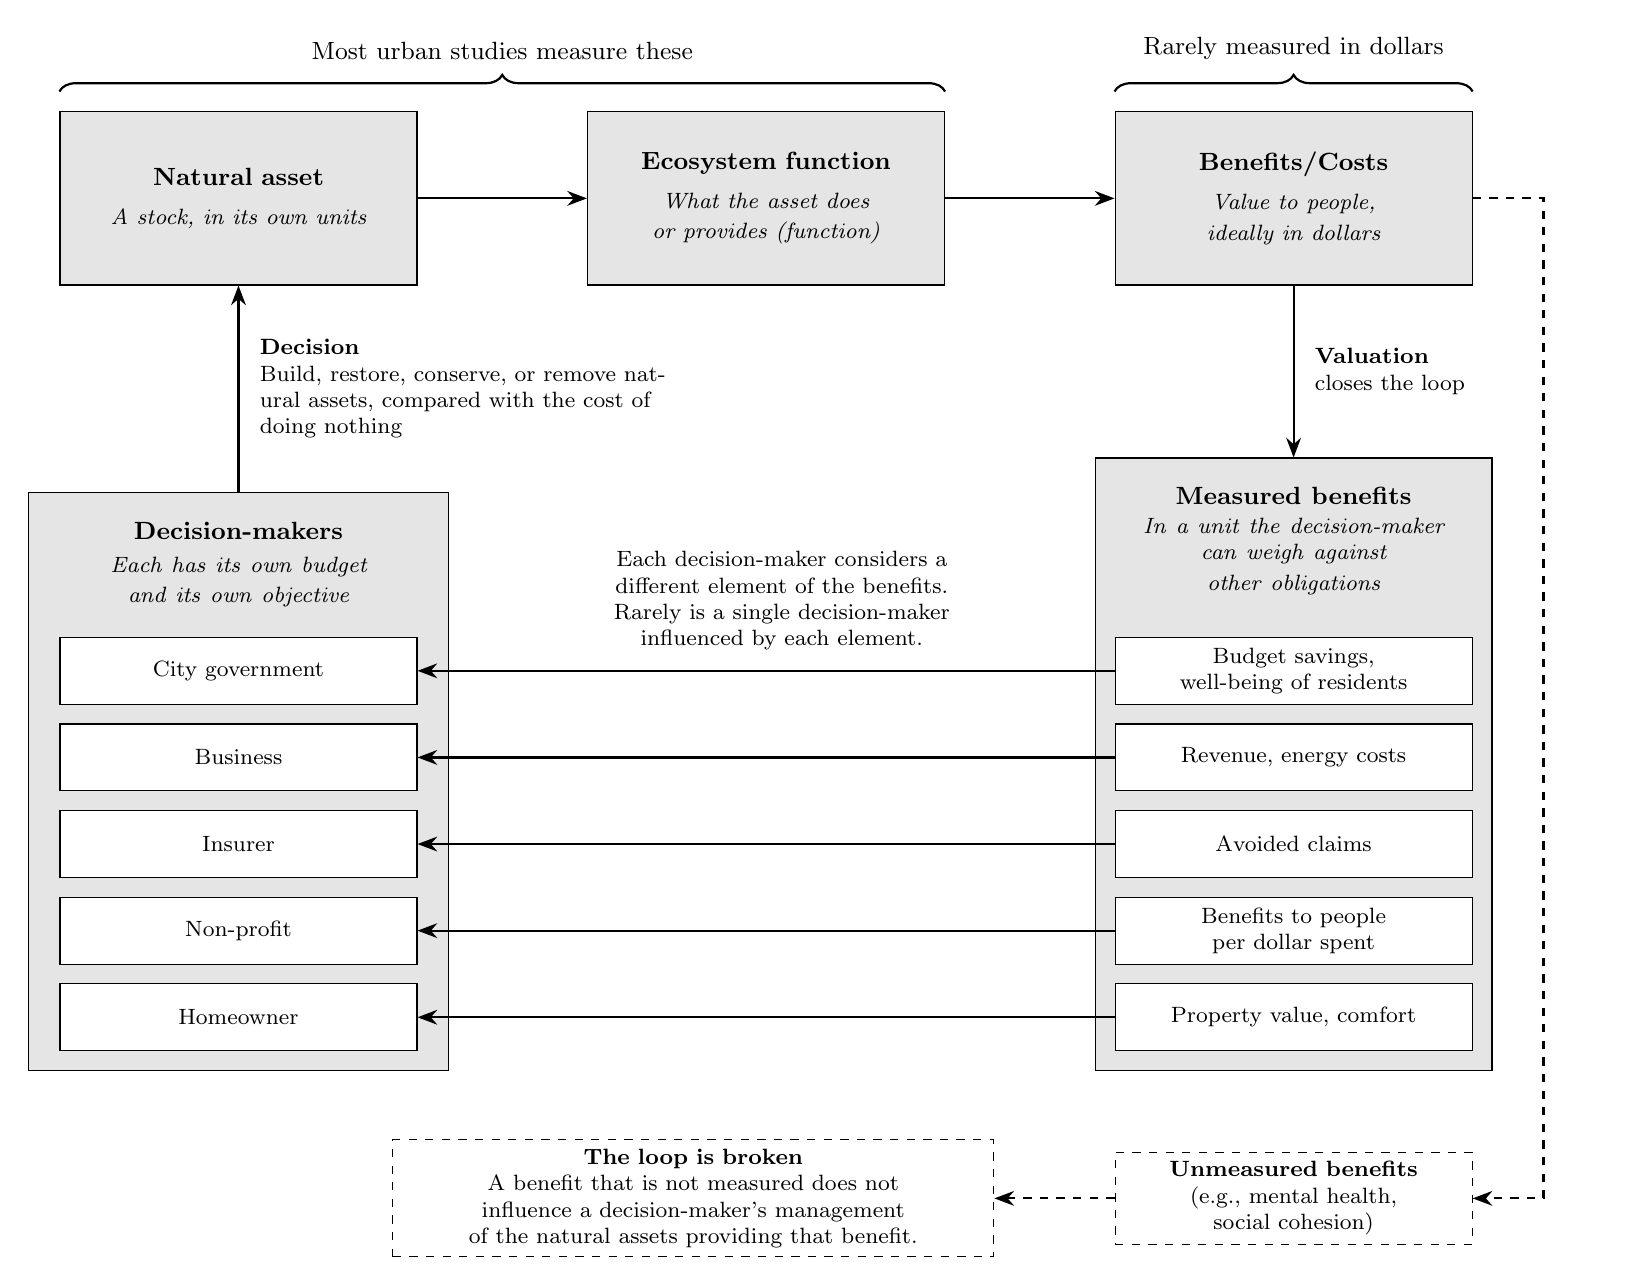
\begin{tikzpicture}[
  font=\small,
  head/.style={draw, fill=gray!20, text width=4.3cm, minimum height=2.2cm, align=center},
  small/.style={draw, fill=white, text width=4.3cm, minimum height=0.85cm, align=center, font=\footnotesize},
  grp/.style={draw, fill=gray!20, inner sep=7pt},
  arr/.style={-{Stealth[length=2.5mm]}, thick},
  lab/.style={align=center, font=\footnotesize}
]
  % ---------------- Top row: how nature produces value ----------------
  \node[head] (a) at (0,0)    {\textbf{Natural asset}\\[3pt]{\footnotesize\itshape A stock, in its own units}};
  \node[head] (s) at (6.7,0)  {\textbf{Ecosystem function}\\[3pt]{\footnotesize\itshape What the asset does or provides (function)}};
  \node[head] (b) at (13.4,0) {\textbf{Benefits/Costs}\\[3pt]{\footnotesize\itshape Value to people, ideally in dollars}};
  \draw[arr] (a) -- (s);
  \draw[arr] (s) -- (b);

  % Where the literature is (braces above the top row)
  \draw[decorate, decoration={brace, amplitude=6pt}, thick]
    ([yshift=0.25cm]a.north west) -- ([yshift=0.25cm]s.north east) node[midway, above=8pt] {Most urban studies measure these};
  \draw[decorate, decoration={brace, amplitude=6pt}, thick]
    ([yshift=0.25cm]b.north west) -- ([yshift=0.25cm]b.north east) node[midway, above=8pt] {Rarely measured in dollars};

  % ---------------- Bottom right: the slice of benefits each decision-maker sees ----------------
  \node[small] (b1) at (13.4,-6.0) {Budget savings,\\well-being of residents};
  \node[small] (b2) at (13.4,-7.1) {Revenue, energy costs};
  \node[small] (b3) at (13.4,-8.2) {Avoided claims};
  \node[small] (b4) at (13.4,-9.3) {Benefits to people\\per dollar spent};
  \node[small] (b5) at (13.4,-10.4) {Property value, comfort};
  \node[font=\small\bfseries, align=center, text width=4.3cm] (bt) at (13.4,-4.35) {Measured benefits\\[1pt]{\footnotesize\mdseries\itshape In a unit the decision-maker\\can weigh against\\other obligations}};
  \begin{scope}[on background layer]
    \node[grp, fit=(bt)(b1)(b5)] (bg) {};
  \end{scope}

  % Unmeasured benefits: the broken loop
  \node[small, dashed, minimum height=1.1cm] (b6) at (13.4,-12.7) {\textbf{Unmeasured benefits}\\(e.g., mental health, social cohesion)};

  % ---------------- Bottom left: decision-makers ----------------
  \node[small] (d1) at (0,-6.0) {City government};
  \node[small] (d2) at (0,-7.1) {Business};
  \node[small] (d3) at (0,-8.2) {Insurer};
  \node[small] (d4) at (0,-9.3) {Non-profit};
  \node[small] (d5) at (0,-10.4) {Homeowner};
  \node[font=\small\bfseries, align=center, text width=4.6cm] (dt) at (0,-4.65) {Decision-makers\\[1pt]{\footnotesize\mdseries\itshape Each has its own budget and its own objective}};
  \begin{scope}[on background layer]
    \node[grp, fit=(dt)(d1)(d5)] (dg) {};
  \end{scope}

  % ---------------- Arrows that close the loop ----------------
  % Valuation: benefits -> measured benefits
  \draw[arr] (b.south) -- (bg.north) node[midway, right=4pt, lab, text width=3.6cm, align=left] {\textbf{Valuation}\\closes the loop};
  % Valuation fails: benefits -> unmeasured
  \draw[arr, dashed] (b.east) -- ++(0.9,0) |- (b6.east);
  % Each slice feeds back to the decision-maker who sees it
  \foreach \i in {1,...,5} { \draw[arr] (b\i.west) -- (d\i.east); }
  \node[lab, fill=white, inner sep=3pt, text width=5.6cm, anchor=south] at (6.9,-5.85) {Each decision-maker considers a\\different element of the benefits.\\Rarely is a single decision-maker\\influenced by each element.};
  % Unmeasured benefits reach no one
  \node[small, dashed, text width=7.4cm, align=center, minimum height=1.1cm, anchor=east] (lb) at (9.6,-12.7) {\textbf{The loop is broken}\\A benefit that is not measured does not\\influence a decision-maker's management\\of the natural assets providing that benefit.};
  \draw[arr, dashed] (b6.west) -- (lb.east);
  % Decision: decision-makers -> natural asset
  \draw[arr] (dg.north) -- (a.south) node[midway, right=4pt, lab, text width=5.4cm, align=left] {\textbf{Decision}\\Build, restore, conserve, or remove natural assets, compared with the cost of doing nothing};
\end{tikzpicture}%
}
\label{fig:concept_framework}

\vspace{0.5em}
\begin{minipage}[t]{0.8\textwidth}
\justifying
\footnotesize \noindent The top row shows how nature produces value: natural assets provide ecosystem functions, which create benefits and costs to people. Most urban studies measure the natural asset and its function \citep{veerkampReviewStudiesAssessing2021}. Far fewer measure the benefit in dollars. The rest of our conceptual framework is organized around the decision. Valuation turns a benefit into a measured benefit, in a unit a decision-maker can weigh against their other obligations. Each decision-maker considers a different element of the measured benefits, and each decides whether to build, restore, conserve, or remove natural assets, compared with the cost of doing nothing. A benefit that is not measured does not feed back into any decision. The decision-makers and benefits listed are illustrative examples, not a complete list.
\end{minipage}
\end{figure}


\subsection{Notes on valuing benefits}
\begin{itemize}
  \item In this framework, valuation is what closes the loop. The point of measuring a benefit is that some decision-maker can act on the number
  \item Direct use (requires you being near/visiting) versus effects you don't need to be close for
  \item Monetized units versus other metrics to well-being
  \item How many people are going to experience the benefits?
  \item Social cohesion is such a hard one to measure at all, but may be a major benefit of parks in cities. How does natural capital build social capital? 
  \item Who receives the benefit, and is that the same as who controls the asset? (links to the decision-maker subsection)
  \item Which benefits matter most to measure: the ones where a decision-maker exists who could act on the number, but the number does not exist yet (e.g., mental health benefits and health insurers)
  \item Measuring perfectly should not be the enemy of measuring at all. A decision-maker needs a number good enough to compare with their other obligations, not a perfect accounting price
\end{itemize}

\subsection{Who is the decision maker?}
\begin{itemize}
  \item Local government
  \item National government
  \item Private sector
  \begin{itemize}
    \item Insurance companies
    \item Storefronts 
    \item Real estate developers
  \end{itemize}
  \item Non-governmental organizations
  \item Home-owners/Neighborhoods
  \item For each decision-maker, the framework asks three things:
  \begin{itemize}
    \item Can they change the stock of natural assets? (Who owns or controls the land?)
    \item Which slice of the benefits do they see? (A storefront sees revenue, an insurer sees claims, a city sees its budget)
    \item Is the one who benefits the same as the one who controls the asset? If not, co-financing or coordination is needed
  \end{itemize}
  \item There is no single ``society'' deciding. This is the main difference from frameworks that close the loop through societal decision-making in aggregate \citep{tanConceptualFrameworkUntangle2020}
  \item Who decides is not always who benefits. This is where distribution enters the framework
\end{itemize}

\subsection{What is the decision maker's objective function?}
\begin{itemize}
  \item No decision-maker is managing for nature alone. Each has its own objective and its own budget, and natural assets compete with everything else in that budget (schools and roads for a city, other investments for a business)
  \item Minimize social disruption 
  \begin{itemize}
    \item Sectors (e.g., transportation, housing, energy, business)
    \item Social groups (e.g., race, income)
  \end{itemize}
  \item Minimize cost
  \begin{itemize}
    \item Energy cost
    \item Healthcare cost
  \end{itemize}
  \item Maximize welfare
  \begin{itemize}
    \item Recreation
    \item Spiritual/Cultural well-being
    \item Social cohesion????
  \end{itemize}
  \item Different decision-makers have different objectives. A city may maximize welfare, a business maximizes profit, an insurer minimizes claims, a non-profit pursues a mission
  \item The objective tells us which unit the benefit has to be measured in for that decision-maker. A benefit that does not enter their objective, or is not measured in their unit, cannot change their decision
\end{itemize}
  
\subsection{What is the relevant counterfactual?}
\begin{itemize}
  \item \textbf{Cities want to know the cost of doing nothing -- that is the relevant counterfactual.} The cost of doing nothing versus the cost of taking action.
  \item This means the framework values a \textit{change} in the stock of natural assets (plant, restore, conserve, or remove), not the total value of everything that exists today
  \item ``Doing nothing'' is not standing still. Cities are growing and the climate is changing, so the baseline moves even without a decision \citep{fenichelEnvironmentalEcosystemServices2025}
  \item The counterfactual also includes the built alternative the decision-maker could pay for instead (air conditioning, seawalls, levees). The value of urban nature is rarely compared with these \citep{keelerSocialecologicalTechnologicalFactors2019}
\end{itemize}




% ------------------------------------------------------------------------------
% A few conceptual/theoretical applications
\section{Theoretical Application of Conceptual Framework}\label{sec:app}
% ------------------------------------------------------------------------------
\begin{itemize}
  \item Apply conceptual framework figure to subset of places 
  \begin{itemize}
    \item Accra, Ghana
    \item New Haven, CT
    \item New York, NY
    \item Burlington, VT
  \end{itemize}
  \item For each place, pick one natural asset and answer the same questions:
  \begin{itemize}
    \item Who can change the stock of this asset?
    \item What are they managing for, and what else competes for their budget?
    \item Which benefits do they see, and in what unit?
    \item What is the cost of doing nothing?
    \item Where is the loop broken? (The benefit is unmeasured, or the one who benefits may not control the asset)
  \end{itemize}
  \item Compare our framework and old conceptual frameworks to show how insights would differ 
  \begin{itemize}
    \item \textbf{This is the test of our contribution.} We need at least one case where our framework leads to a different conclusion than the cascade would (e.g., the function is well measured, but no asset gets built because no decision-maker sees the benefit)
    \item My current concern is without a solid example a reviewer could say the framework is just benefit-cost analysis / nothing that Tan et al.\ didn't say
  \end{itemize}
  \item Maybe some simple statistics about number of people benefiting from certain ecosystem services, distributions, how those stats have changed over time to emphasize the dynamic aspect of framework 
\end{itemize}

% ------------------------------------------------------------------------------
% Next steps/research agenda 
\section{Going Forward}\label{sec:next}
% ------------------------------------------------------------------------------
\begin{itemize}
  \item What data and modeling needs to be done to operationalize this CF 
  \begin{itemize}
    \item Which natural assets are already well mapped? Which functions do we already have strong certainty around?
    \item Which benefits do we hypothesize are large to some decision-maker, and how would we go measure that?
    \item Some of this could come from Andie's review
  \end{itemize}
  \item Which stakeholders need to be engaged to implement this CF
  \begin{itemize}
    \item The stakeholders are the decision-makers in the framework. Ask them directly what they are managing for and what number would change their decision
  \end{itemize}
  \item Slight outline of research agenda 
  \begin{itemize}
    \item The framework sets the priorities: measure the benefits where a decision-maker exists who could act on the number, but the number does not exist yet
    \item Which arrows in the figure are we working on, and which are important but not our focus?
  \end{itemize}
\end{itemize}



\newpage
\bibliographystyle{aer}
\bibliography{../references}

\end{document}
